\documentclass[journal,12pt,twocolumn]{IEEEtran}
%
\usepackage{setspace}
\usepackage{gensymb}
\usepackage{siunitx}
\usepackage{tkz-euclide} 
\usepackage{textcomp}
\usepackage{standalone}
\usetikzlibrary{calc}

%\doublespacing
\singlespacing

%\usepackage{graphicx}
%\usepackage{amssymb}
%\usepackage{relsize}
\usepackage[cmex10]{amsmath}
%\usepackage{amsthm}
%\interdisplaylinepenalty=2500
%\savesymbol{iint}
%\usepackage{txfonts}
%\restoresymbol{TXF}{iint}
%\usepackage{wasysym}
\usepackage{amsthm}
%\usepackage{iithtlc}
\usepackage{mathrsfs}
\usepackage{txfonts}
\usepackage{stfloats}
\usepackage{bm}
\usepackage{cite}
\usepackage{cases}
\usepackage{subfig}
%\usepackage{xtab}
\usepackage{longtable}
\usepackage{multirow}
%\usepackage{algorithm}
%\usepackage{algpseudocode}
\usepackage{enumitem}
\usepackage{mathtools}
\usepackage{steinmetz}
\usepackage{tikz}
\usepackage{circuitikz}
\usepackage{verbatim}
\usepackage{tfrupee}
\usepackage[breaklinks=true]{hyperref}
%\usepackage{stmaryrd}
\usepackage{tkz-euclide} % loads  TikZ and tkz-base
%\usetkzobj{all}
\usetikzlibrary{calc,math}
\usepackage{listings}
    \usepackage{color}                                            %%
    \usepackage{array}                                            %%
    \usepackage{longtable}                                        %%
    \usepackage{calc}                                             %%
    \usepackage{multirow}                                         %%
    \usepackage{hhline}                                           %%
    \usepackage{ifthen}                                           %%
  %optionally (for landscape tables embedded in another document): %%
    \usepackage{lscape}     
\usepackage{multicol}
\usepackage{chngcntr}
\usepackage{amsmath}
\usepackage{cleveref}
%\usepackage{enumerate}

%\usepackage{wasysym}
%\newcounter{MYtempeqncnt}
\DeclareMathOperator*{\Res}{Res}
%\renewcommand{\baselinestretch}{2}
\renewcommand\thesection{\arabic{section}}
\renewcommand\thesubsection{\thesection.\arabic{subsection}}
\renewcommand\thesubsubsection{\thesubsection.\arabic{subsubsection}}

\renewcommand\thesectiondis{\arabic{section}}
\renewcommand\thesubsectiondis{\thesectiondis.\arabic{subsection}}
\renewcommand\thesubsubsectiondis{\thesubsectiondis.\arabic{subsubsection}}

% correct bad hyphenation here
\hyphenation{op-tical net-works semi-conduc-tor}
\def\inputGnumericTable{}                                 %%

\lstset{
%language=C,
frame=single, 
breaklines=true,
columns=fullflexible
}
%\lstset{
%language=tex,
%frame=single, 
%breaklines=true
%}
\usepackage{graphicx}
\usepackage{pgfplots}

\begin{document}
%


\newtheorem{theorem}{Theorem}[section]
\newtheorem{problem}{Problem}
\newtheorem{proposition}{Proposition}[section]
\newtheorem{lemma}{Lemma}[section]
\newtheorem{corollary}[theorem]{Corollary}
\newtheorem{example}{Example}[section]
\newtheorem{definition}[problem]{Definition}
%\newtheorem{thm}{Theorem}[section] 
%\newtheorem{defn}[thm]{Definition}
%\newtheorem{algorithm}{Algorithm}[section]
%\newtheorem{cor}{Corollary}
\newcommand{\BEQA}{\begin{eqnarray}}
\newcommand{\EEQA}{\end{eqnarray}}
\newcommand{\define}{\stackrel{\triangle}{=}}
\bibliographystyle{IEEEtran}
%\bibliographystyle{ieeetr}
\providecommand{\mbf}{\mathbf}
\providecommand{\pr}[1]{\ensuremath{\Pr\left(#1\right)}}
\providecommand{\qfunc}[1]{\ensuremath{Q\left(#1\right)}}
\providecommand{\sbrak}[1]{\ensuremath{{}\left[#1\right]}}
\providecommand{\lsbrak}[1]{\ensuremath{{}\left[#1\right.}}
\providecommand{\rsbrak}[1]{\ensuremath{{}\left.#1\right]}}
\providecommand{\brak}[1]{\ensuremath{\left(#1\right)}}
\providecommand{\lbrak}[1]{\ensuremath{\left(#1\right.}}
\providecommand{\rbrak}[1]{\ensuremath{\left.#1\right)}}
\providecommand{\cbrak}[1]{\ensuremath{\left\{#1\right\}}}
\providecommand{\lcbrak}[1]{\ensuremath{\left\{#1\right.}}
\providecommand{\rcbrak}[1]{\ensuremath{\left.#1\right\}}}
\theoremstyle{remark}
\newtheorem{rem}{Remark}
\newcommand{\sgn}{\mathop{\mathrm{sgn}}}
\providecommand{\abs}[1]{\left\vert#1\right\vert}
\providecommand{\res}[1]{\Res\displaylimits_{#1}} 
\providecommand{\norm}[1]{\left\lVert#1\right\rVert}
%\providecommand{\norm}[1]{\lVert#1\rVert}
\providecommand{\mtx}[1]{\mathbf{#1}}
\providecommand{\mean}[1]{E\left[ #1 \right]}
\providecommand{\fourier}{\overset{\mathcal{F}}{ \rightleftharpoons}}
%\providecommand{\hilbert}{\overset{\mathcal{H}}{ \rightleftharpoons}}
\providecommand{\system}{\overset{\mathcal{H}}{ \longleftrightarrow}}
	%\newcommand{\solution}[2]{\textbf{Solution:}{#1}}
\newcommand{\solution}{\noindent \textbf{Solution: }}
\newcommand{\cosec}{\,\text{cosec}\,}
\providecommand{\dec}[2]{\ensuremath{\overset{#1}{\underset{#2}{\gtrless}}}}
\newcommand{\myvec}[1]{\ensuremath{\begin{pmatrix}#1\end{pmatrix}}}
\newcommand{\mydet}[1]{\ensuremath{\begin{vmatrix}#1\end{vmatrix}}}
%\numberwithin{equation}{section}
\numberwithin{equation}{subsection}
%\numberwithin{problem}{section}
%\numberwithin{definition}{section}
\makeatletter
\@addtoreset{figure}{problem}
\makeatother
\let\StandardTheFigure\thefigure
\let\vec\mathbf
%\renewcommand{\thefigure}{\theproblem.\arabic{figure}}
\renewcommand{\thefigure}{\theproblem}
%\setlist[enumerate,1]{before=\renewcommand\theequation{\theenumi.\arabic{equation}}
%\counterwithin{equation}{enumi}
%\renewcommand{\theequation}{\arabic{subsection}.\arabic{equation}}
\def\putbox#1#2#3{\makebox[0in][l]{\makebox[#1][l]{}\raisebox{\baselineskip}[0in][0in]{\raisebox{#2}[0in][0in]{#3}}}}
     \def\rightbox#1{\makebox[0in][r]{#1}}
     \def\centbox#1{\makebox[0in]{#1}}
     \def\topbox#1{\raisebox{-\baselineskip}[0in][0in]{#1}}
     \def\midbox#1{\raisebox{-0.5\baselineskip}[0in][0in]{#1}}
\vspace{3cm}
\title{Matrix Theory (EE5609) Assignment 8}
\author{Arkadipta De\\MTech Artificial Intelligence\\AI20MTECH14002}

\maketitle
\newpage
%\tableofcontents
\bigskip
\renewcommand{\thefigure}{\theenumi}
\renewcommand{\thetable}{\theenumi}

\begin{abstract}
This document finds what conic section a given second degree equation represent.
\end{abstract}

All the codes for the figure in this document can be found at
\begin{lstlisting}
https://github.com/Arko98/EE5609/blob/master/Assignment_8
\end{lstlisting}

\section{Problem}
What conic does the following equation represent. 
\begin{align*}
13x^2-18xy+37y^2+2x+14y-2 = 0
\end{align*}
Find the center.
\section{Solution}
The general second degree equation can be expressed as follows,
\begin{align}
\vec{x^T}\vec{V}\vec{x}+2\vec{u^T}\vec{x}+f=0\label{eqmain}
\end{align}
From the given second degree equation we get,
\begin{align}
\vec{V} &= \myvec{13&-9\\-9&37}\\
\vec{u} &= \myvec{1\\7}\\
f &= -2
\end{align}
Expanding the determinant of $\vec{V}$ we observe, 
\begin{align}
\mydet{13&-9\\-9&37} = 400>0 \label{eqV}
\end{align}
Hence from \eqref{eqV} we conclude that given equation is an ellipse. The characteristic equation of $\vec{V}$ is given as follows,
\begin{align}
\mydet{\lambda\vec{I}-\vec{V}} = \mydet{\lambda-13&9\\9&\lambda-37} &= 0\\
\implies \lambda^2-50\lambda+400 &= 0\label{eqchar}
\end{align}
Hence the characteristic equation of $\vec{V}$ is given by \eqref{eqchar}. The roots of \eqref{eqchar} i.e the eigenvalues are given by
\begin{align}
\lambda_1=10, \lambda_2=40\label{eqeigenvals}    
\end{align}
The eigen vector $\vec{p}$ is defined as, 
\begin{align}
\vec{V}\vec{p} &= \lambda\vec{p}\\
\implies\brak{\lambda\vec{I}-\vec{V}}\vec{p}&=0
\end{align}
for $\lambda_1=10$,
\begin{align}
\brak{\lambda_1\vec{I}-\vec{V}}&=\myvec{-3&9\\9&-27}\xleftrightarrow[R_1=\frac{1}{3}R_1]{R_2=R_2+3R_1}\myvec{-1&3\\0&0}\\
\implies\vec{p_1}&=\myvec{3\\1}
\end{align}
Again, for $\lambda_2=40$,
\begin{align}
\brak{\lambda_2\vec{I}-\vec{V}}&=\myvec{27&9\\9&3}\xleftrightarrow[R_1=\frac{1}{27}R_1]{R_2=R_2-R_1}\myvec{1&\frac{1}{3}\\0&0}\\
\implies\vec{p_2}=\myvec{-1\\3}
\end{align}
Again, 
Hence from the equation
\begin{align}
\vec{V}&=\vec{P}\vec{D}\vec{P^{-1}}
\intertext{Where $\vec{D}$ is a diagonal matrix, we get,}
\vec{P}&=\myvec{\vec{p_1}&\vec{p_2}}=\myvec{3&-1\\1&3}\\
\vec{D}&=\myvec{10&0\\0&40}
\end{align}
Now \eqref{eqmain} can be written as,
\begin{align}
\vec{y^T}\vec{D}\vec{y}&=\vec{u^T}\vec{V^{-1}}\vec{u}-f\qquad\text{$\mydet{\vec{V}}\not=0$}\label{eqnewmain}\\
\intertext{And,}
\vec{c}&= -\vec{V^{-1}}\vec{u}\qquad\text{$\mydet{\vec{V}}\not=0$}\label{eqcenter}\\
\vec{y} &= \vec{P^T}\brak{\vec{x-c}}\label{eqY}
\end{align}
The centre/vertex of the conic section in \eqref{eqmain} is given by $\vec{c}$ in \eqref{eqcenter}. 
We compute $\vec{V^{-1}}$ as follows,
\begin{align}
\myvec{13&-9&1&0\\-9&37&0&1}&\xleftrightarrow[R_2=\frac{13}{400}R_2]{R_2=R_2+\frac{9}{13}R_1}\myvec{13&-9&1&0\\0&1&\frac{9}{400}&\frac{13}{400}}\\
&\xleftrightarrow[R_1=R_1+\frac{9}{13}R_2]{R_1=\frac{1}{13}R_1}\myvec{1&0&\frac{37}{400}&\frac{9}{400}\\0&1&\frac{9}{400}&\frac{13}{400}}
\end{align}
Hence $\vec{V^{-1}}$ is given by,
\begin{align}
\vec{V^{-1}} = \myvec{\frac{37}{400}&\frac{9}{400}\\\frac{9}{400}&\frac{13}{400}}
\end{align}
Now $\vec{u^T}\vec{V^{-1}}\vec{u}$ is given by,
\begin{align}
\vec{u^T}\vec{V^{-1}}\vec{u}&=\frac{1}{400}\myvec{1&7}\myvec{37&9\\9&13}\myvec{1\\7}=2\label{eqRHS}\\
\intertext{And, $\vec{V^{-1}}\vec{u}$ is given by,}
\vec{V^{-1}}\vec{u} &= \frac{1}{400}\myvec{100\\100}=\frac{1}{4}\myvec{1\\1}\label{eqcenterRHS}
\end{align}
By putting the value of \eqref{eqcenterRHS}, the center of the ellipse is given by \eqref{eqcenter} as follows,
\begin{align}
\myvec{x_c\\y_c} = -\frac{1}{4}\myvec{1\\1} = \myvec{-\frac{1}{4}\\-\frac{1}{4}}
\end{align}
Also the semi-major axis ($a$) and semi-minor axis ($b$) of the ellipse are given by,
\begin{align}
a = \sqrt{\frac{\vec{u^T}\vec{V^{-1}}\vec{u}-f}{\lambda_1}}=\frac{\sqrt{10}}{5}\\
b = \sqrt{\frac{\vec{u^T}\vec{V^{-1}}\vec{u}-f}{\lambda_2}}=\frac{\sqrt{10}}{10}
\end{align}
Again, $\vec{y}$ from \eqref{eqY} is given by,
\begin{align}
\vec{y} &= \myvec{3&-1\\1&3}\myvec{x+\frac{1}{4}\\y+\frac{1}{4}}\label{eqNew}
\end{align}
Finally putting values from \eqref{eqRHS} and \eqref{eqNew} in \eqref{eqnewmain}, the equation of ellipse is given by,
\begin{align}
&\vec{y^T}\myvec{10&0\\0&40}\vec{y}=4\label{eqFinal}
\end{align}

The following figure is the graphical representation of the ellipse in \eqref{eqFinal},
\renewcommand{\thefigure}{1}
\begin{figure}[h!]
\centering
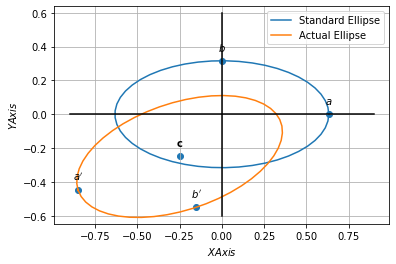
\includegraphics[width = \columnwidth]{Ellipse.png}
\caption{Graphical representation of the ellipse}
\label{fig:my_label}
\end{figure}

\end{document}